\documentclass[12pt]{article}
\usepackage[bottom=2cm,top=2cm,left=2.5cm,right=2.5cm]{geometry}
\usepackage{amsmath}
\allowdisplaybreaks
%\usepackage{amsmath} %%% Biblio de math\'ematiques
\usepackage{amssymb} %%% Biblio de math\'ematiques
\usepackage{lmodern} %%% Pour que les accents soient correconstantement trait\'es dans le PDF
\usepackage[table]{xcolor} %%% Coloriage
\usepackage{mathtools} %%% Pour les maths
\usepackage{xspace} %%% Pour espacer de fa\'eon correct
\usepackage{fancybox} %%% Encadrement
\usepackage{graphicx} %%% Espacement control\'e!
\usepackage{thmtools} %%% Biblio de maths
\usepackage{mathrsfs}%%%\mathscr
\usepackage{booktabs}
\usepackage[english]{babel}
\usepackage{bm}
%\usepackage{frcursive} %%% Ecrire caligraphique
\usepackage{mathrsfs}%%%\mathscr
\usepackage{booktabs}
\usepackage{hyperref}
%\usepackage{isomath,bbold}%{omlmathbf,omlmathit,omlmathrm,omlmathsfit,mathsfbf,,pzcal}
\usepackage{amsmath} %%% Biblio de math\'ematiques
\usepackage{amssymb} %%% Biblio de math\'ematiques
\usepackage{lmodern} %%% Pour que\Opes accents soient correconstantement trait\'es dans\Ope

%\usepackage{frcursive} %%% Ecrire caligraphique
\usepackage{mathrsfs}%%%\mathscr
\usepackage{microtype}


%% -- Figures & tableaux -------------------------------------
\usepackage{graphicx,float,booktabs,multirow,tabularx,array,longtable}
\usepackage[font=small,labelfont=bf,justification=centering]{caption}
\usepackage{subcaption}
\usepackage{xcolor,colortbl}


\definecolor{darkblue}{RGB}{0,50,110}
\definecolor{lightblue}{RGB}{215,232,250}
\definecolor{lightyellow}{RGB}{255,251,210}
\definecolor{lightgreen}{RGB}{218,245,218}
\definecolor{lightgray}{RGB}{242,242,242}
\definecolor{myorange}{RGB}{210,90,20}
\definecolor{mygray}{RGB}{100,100,100}
\definecolor{darkred}{RGB}{140,20,20}

%% -- TikZ --------------------------------------------------
\usepackage{listings}
\usepackage{tikz}
\usetikzlibrary{shapes.geometric,arrows.meta,positioning,
	fit,backgrounds,shadows,calc,
	decorations.pathreplacing,decorations.markings}

\tikzset{
	src/.style    = {rectangle,rounded corners=3pt,draw=darkblue,
		fill=lightblue,minimum width=2.3cm,
		minimum height=0.7cm,align=center,
		font=\small\sffamily,drop shadow},
	proc/.style   = {rectangle,draw=myorange!80,fill=lightyellow,
		minimum width=5cm,minimum height=0.7cm,
		align=center,font=\small\sffamily,drop shadow},
	stor/.style   = {cylinder,shape border rotate=90,aspect=0.28,
		draw=darkblue!60,fill=lightgreen,
		minimum width=1.8cm,minimum height=0.95cm,
		align=center,font=\small\sffamily},
	outb/.style   = {rectangle,rounded corners=3pt,draw=purple!60,
		fill=purple!10,minimum width=2.1cm,
		minimum height=0.7cm,align=center,
		font=\small\sffamily,drop shadow},
	qa/.style     = {rectangle,draw=darkred!60,fill=red!7,
		minimum width=5cm,minimum height=0.7cm,
		align=center,font=\small\sffamily},
	dagnode/.style= {circle,draw=darkblue,fill=lightblue!70,
		minimum size=0.9cm,align=center,
		font=\scriptsize\sffamily},
	arr/.style    = {-{Stealth[scale=1.1]},thick,darkblue},
	qarr/.style   = {-{Stealth[scale=1.0]},thick,myorange,dashed},
}

%% -- pgfplots -----------------------------------------------
\usepackage{pgfplots}
\pgfplotsset{compat=1.18}
\usepackage{pgfplotstable}


\usepackage{enumitem}
\usepackage{tcolorbox}
\tcbuselibrary{skins,breakable,theorems}
\usepackage{fancyhdr}
\usepackage{titlesec}
\usepackage{appendix}
\usepackage{algorithm}
\usepackage{algorithmic}

\newtcolorbox{contribbox}{
	colback=lightblue!60,colframe=darkblue,
	title={\sffamily\bfseries Contributions principales},
	fonttitle=\small,left=4pt,right=4pt,top=4pt,bottom=4pt,
	breakable}

\newtcolorbox{resultbox}{
	colback=lightgreen!60,colframe=darkblue!60,
	left=4pt,right=4pt,top=4pt,bottom=4pt,boxrule=0.5pt,
	breakable}

\newtcolorbox{mathbox}[1]{
	colback=lightyellow!80,colframe=myorange!70,
	title={\sffamily\small #1},
	left=4pt,right=4pt,top=3pt,bottom=3pt,
	breakable}

\pagestyle{fancy}
\fancyhf{}
\fancyhead[L]{\small\sffamily\color{mygray}
	AgriFlow -- Orchestration de pipelines spatio-temporels heterogenes}
\fancyhead[R]{\small\sffamily\color{mygray}\thepage}
\renewcommand{\headrulewidth}{0.4pt}


%%%%%%%%%%%%%%%%%%%%%%%%%%%%%%%%%%%%%%%% TITLE %%%%%%%%%%%%%%%%%%%%%%
\title{\rm Agriflow Formally-Founded Orchestration Framework for Heterogeneous Spatio-Temporal Data Pipeline in Precision Agriculture.}
\author{IssakaLouk-Man$^{a,b}$ }
%\footnote{E-mail address : issaka.louk-man@ugb.edu.sn}, Amadou Diop $^a$\footnote{E-mail address : diop.amadou@ugb.edu.sn}}
\date{\today}

%%%%%%%%%%%%%%%%%%%%%%%%%%%%%%%%%%%%%%%%%%%%%%%%%%%%%%%%%%%%%%%%% %%%%%%%%
\newtheorem{theorem}{Theorem}[section]
\newtheorem{proposition}{Proposition}[section]
\newtheorem{corollary}[theorem]{Corollary}
\newtheorem{lemma}[theorem]{Lemma}
\newtheorem{example}{Example}[section]
\newtheorem{definition}{Definition}[section]
\newtheorem{remark}{Remark}[section]
\newenvironment{proof}{$\mathbf{Proof.\quad}$}{\begin{flushright}$\bigstar$\end{flushright}}

\usepackage{mathtools}
\DeclarePairedDelimiter\ceil{\lceil}{\rceil}
\DeclarePairedDelimiter\floor{\lfloor}{\rfloor}
\DeclareMathOperator{\diam}{diam}
\DeclareMathOperator{\ent}{H}
\DeclareMathOperator{\KL}{KL}
\DeclareMathOperator{\MI}{I}
\DeclareMathOperator{\rank}{rang}
\newcommand{\E}{\mathbb{E}}
\newcommand{\R}{\mathbb{R}}
\newcommand{\N}{\mathbb{N}}
\newcommand{\Prob}{\mathbb{P}}
\newcommand{\indic}{\mathbf{1}}
\newcommand{\norm}[1]{\left\|#1\right\|}
\newcommand{\abs}[1]{\left|#1\right|}
\newcommand{\inner}[2]{\langle #1,\, #2 \rangle}

%% -- Figures & tableaux -------------------------------------
\usepackage{graphicx,float,booktabs,multirow,tabularx,array,longtable}
\usepackage[font=small,labelfont=bf,justification=centering]{caption}
\usepackage{subcaption}
\usepackage{xcolor,colortbl}
\begin{document}
\newcommand{\Bc}{\mathscr{B}}
\newcommand{\Vilbert}{\mathcal{V}}
\newcommand{\Xilbert}{\mathbf{X}}
\newcommand{\Kilbert}{\mathbf{K}}

\fontsize{12pt}{23pt}\selectfont

\maketitle
{\footnotesize
	\begin{flushleft}
		\hspace{1cm}\thanks{$^a$ Institut de Mathématiques de Toulouse, Université Paul Sabatier, 118 route de Narbonne, 31062 \\
			\hspace{1.5cm}Toulouse Cedex 9, France}\\
		\hspace{1cm}\thanks{$^a$ Laboratoire d'Analyse num\'{e}rique et informatique, UFR SAT, D\'{e}partement de Math\'{e}matiques,\\
			\hspace{1.5cm} Universit\'{e} Gaston Berger de Saint-Louis, S\'{e}n\'{e}gal}\\
\end{flushleft}}
\begin{abstract}
	L'intégration de flux de données hétérogènes issus de capteurs IoT, d'imagerie Sentinel-2 et des systèmes FMIS au sein de pipeline analytique fiables représente un défi majeur pour l'agriculture de précision (PA). Les solutions ad hoc actuelles manquent de formalisme entraînant des architectures fragiles et une dégradation silencieuse de la qualité des données.   Cet article introduit \textbf{AgriFlow}, un modèle  d'orchestration robuste et formalisé pour l'agriculture numérique basé sur Apache Airflow.  Nos contributions incluent un modele de graphe orienté acyclique (DAG) fortement typé pour les chaines de traitement spatio-temporelle;  un mecanisme de propagation de la qualité compositionnelle ($Q_j=q_j\cdot \Pi_{i} Q_i^{w_{ij}}$), avec des bornes de sensibilité théorique; et, un opérateur d'alignement spatio-temporel $\mathcal{A}$. Ce cadre a été validé par une simulation de Monte Carlo sur 365 jours ($N=1000$).  Les résultat démontrent une fiabilité d’exécution de $96,7\pm7,2\%$ surpassant significativement les scripts classiques ($p< 0,001$). De plus, les bornes de sensibilité théorique ont été validé avec une erreur relative minimale de $0,23\%$ confirmant la précision du modèle formel proposé.
\end{abstract}



{\textbf{Keywords:} ETL pipeline, quality propagation, spatio-temporal operator, Apache Airflow, information theory }\\
{\textbf{Mathematics Subject Classifcation :} \%\%\%\%\%\%\%.}
%%%%%%%%%%%%%%%%%%%%%%%%%%%%%%%%%%%%%%%%%%%%%%%%%%%%%%%%%%%%
\renewcommand{\baselinestretch}{1.05}
\newcommand{\SAP}{\mathcal{S}A_{\omega\mathcal{Q}}P\left(\mathbb{X}\right)}
\newcommand{\SAPO}{\mathcal{S}A_{\omega\mathcal{Q},0}P\left(\mathbb{X}\right)}
\newcommand{\BC}{BC(\mathbb{R}^+,\mathbb{X})}

\section{Introduction}
La digitalisation de l'agriculture a engendré une prolifération de source de données hétérogènes.   Dans les déploiement d'agriculture de précision,la surveillance d'une parcelle repose sur une synergie des données IoT (TDR/FDR), de l'imagerie satellitaire (Sentinel-2), des APIs météorologiques et des systèmes de gestion agricole (FMIS). Si l'exploitation conjointe de ces sources est necessaire pour mettre en place des modèles de culture spatialement explicite, leurs intégration au sein des pipelines analytique reste un défi majeur. \\

Les pratiques habituelles utilisent des scriptes ad hoc qui se limités en dépendance et à la tolérance liées aux pannes.  Il est aussi sans doute, de constaté que ces pratiques souffrent de défaillances <<silencieuse>> (une corruption de donnée ou une modification de schéma d'API peut altérer l'intégrité de la chaîne décisionnelle sans d'alerte explicite\cite). Nos scenarios de simulation basé sur des cas d'usage réels (UC3) illustre ce risque (l'injection d'une anomalie non détectée dans un flux FMIS engendre une chute du coefficient de détermination ($R^2$) du modèle de prédiction de $0,81$ à $0,61$ en quatre semaine compromettant gravement la fiabilité de décision d'irrigation).

Au cours de ces dernières décennies, l'orchestration de workflow via les outils comme Apache Airflow  révolutionné plusieurs domaine comme finance \cite{}, télécommunication \cite{}, bio-informatique \cite{},  etc.. Pourtant, son application rigoureuse rigoureuse reste absente dans le  domaine informatique agricole. Dans la littérature actuelle, il n'existe pas un formalisme unifiant l'orchestration de pipeline complexes et la propagation théorique de la qualité des données.  Pour combler ce manque, cet article présente, AgriFlow, un cadre d'orchestration robuste ancré dans un modèle algébrique formel. Les principales contributions de travail sont les suivantes:
\begin{enumerate}
	\item \textbf{Modélisation algébrique:} Nous présentons des pipelines comme des Graphes Orientés Acyclique à typage fort, où chaque n\oe ud intègre des métriques de qualité fondées
	sur la théorie de l’information.
	\item \textbf{Mécanisme de propagation de la qualité :} Nous introduisons une loi compositionnelle ($Q_j = q_j \cdot \prod Q_i^{w_{ij}}$) donnant un théorème de monotonicité et de calculs de sensibilité analytique  ($\partial Q_j / \partial Q_i$)
	\item \textbf{Implémentation et Alignement :} Le cadre est implémenté sur Apache Airflow
	$2.7$, intégrant un opérateur d’alignement spatio-temporel ($\mathcal{A}$) garantissant la cohérence 	sémantique des données fusionnées.
	\item \textbf{Validation par simulation :} Une évaluation exhaustive par simulation de Monte Carlo ($N=1\,000$ réplications sur 365 jours) démontre une fiabilité d'exécution de $96,7 \pm 7,2\,\%$. La précision du modèle de sensibilité est confirmée par une erreur relative de seulement $0,23\,\%$.
	
\end{enumerate}
La suite de ce travail est organisé comme suit: Dans la section \ref{sect2}

\section{Etat de l'art}\label{sect2} 
\label{sec:related}
%%===========================================================

\subsection{Integration de donnees heterogenes en agriculture de precision}

\paragraph{Caractérisation des donnée in situ : capteurs IoT}

Les capteurs IoT déployés en parcelle représentent la couche de données la plus opérationnelle de l’Agriculture de Précision. Les sondes d'humidité volumique (TDR,FDR), les capteurs de conductivité électrique apparente ($\text{EC}_a$) et les thermocouples alimentent des passerelles LPWAN (LoRaWAN, Sigfox) ou cellulaires (4G/LTE) transmettant les relevés via MQTT ou HTTPS \cite{iot_review_2025,iot_frontiers_2025}. La principale difficulté réside dans la normalisation de ces flux : chaque fabricant utilise des unités, des gammes et des protocoles distincts
\cite{iot_agronomy_2023}. Sur le plan stochastique, les séries temporelles
IoT agricoles présentent des lacunes non aléatoires : les coupures de connectivité sont corrélée au climat (orages) et a la topographie (masques radios), ce qui invalide les hypothèses d’erreurs aléatoires
indépendantes des modèles d'imputation classiques.

\paragraph{Télédétection satellite : Sentinel-2.} Lancé dans le cadre du programme Copernicus depuis, Sentinel-2 a pour mission de fournir des images multispectrales a 10 -- 60 ~m de résolution spatiale et $5$ jours de revisite en Europe \cite{sentinel2_ard_2022}. Les produits de données sont librement accessibles via le Copernicus Data Space Ecosystem (CDSE). Les indices dérivés (
$\text{NDVI} = (\rho_{NIR}-\rho_{Red})/(\rho_{NIR}+\rho_{Red})$,
$\text{NDWI} = (\rho_{Green}-\rho_{NIR})/(\rho_{Green}+\rho_{NIR})$,
LAI, EVI ) constituent les variables d'état phytosanitaire de référence \cite{ndvi_sentinel2_2023,ndvi_timeseries_2022}.
La couverture nuageuse constitue la principale limitation : en Europe
tempérée, jusqu'a 60\,\% des acquisitions automnales sont inutilisables,
introduisant des lacunes corrolées dans les séries NDVI. Ces lacunes
brisent les hypothèses de stationnarité requises par les détecteurs
d'anomalie classiques, ce qui motive notre stratégie de masquage SCL
et d'interpolation temporelle (Section~\ref{subsec:alignment_impl}).

\paragraph{Interopérabilité et alignement spatio-temporel}
L'exploitation conjointe de capteurs IoT et de données de satellite requiert
la résolution de trois problèmes d'alignement fondamentaux :
\begin{itemize}
	\item [(i)] l'alignement \emph{spatial} : les capteurs fournissent des mesures
ponctuelles et les satellites des valeurs surfaciques : le changement
de support (change of support problem, COSP) est un problème géo-statistique
ouvert \cite{change_of_support} ;
\item [(ii)]~l'alignement \emph{temporel} : les deux sources opèrent sur des
grilles temporelles incompatibles (30~min vs 5~j) ;
\item [(iii)]l'alignement \emph{systémique de référence} : la dispersion
entre projections geographiques (WGS84, Lambert 93, etc.) produit des
biais de co-registration pouvant atteindre 40~m, supérieur a un pixel
Sentinel-2.
\end{itemize}

\subsection{Approches ETL existantes pour les données agricoles}

Les solutions d’intégration existantes se repartissent en trois catégories.
Les \textbf{outils SIG spécialisés} (FME Safe Software, extensions ETL
de QGIS) supportent l'intégration de formats géospatiaux hétérogènes
mais ne disposent d'aucune capacité de scheduling, de retry ni de
monitoring \cite{fme_agri}.
Les \textbf{plateformes analytiques cloud} (Google Earth Engine,
Microsoft Planetary Computer) offrent une puissance de calcul satellite
exceptionnelle mais imposent un enfermement propriétaire et n’intègrent
pas les flux locaux IoT ou FMIS \cite{gee_agriculture}.
Les \textbf{scripts ad hoc} (pratique dominante)  permettent un
prototypage rapide mais ne passent pas a l’échelle et ne fournissent
aucune reproductibilité ni tolérance aux pannes \cite{pipeline_survey_2024}.
Aucune de ces approches ne fournit un cadre monitorable et formellement
fonde pour l'intégration multi-sources agricoles.

\subsection{Orchestration de workflows scientifiques}

Apache Airflow \cite{airflow_docs}, publie sous licence Apache 2.0 par
Airbnb en 2014 et intègre a l'Apache Software Foundation en 2016, est
devenu le standard de facto pour les pipelines de données intensives.
Son abstraction centrale, le DAG, modèle naturellement les dépendances
entre tâches ETL : les n\oe uds représentent des opérations atomiques
(opérateurs) et les arêtes encodent les flux de données.
Airflow supporte nativement plus de 1000 opérateurs couvrant HTTP,
SQL, Kubernetes, Python et des extensions spécifiques au domaine.
Depuis la version 2.7, les Datasets permettent un déclenchement basé
sur évènements qui élimine le besoin d'interrogation (polling)
\cite{airflow_docs}.

Prefect et Luigi constituent des alternatives compétitives pour les
workflows legers. Nextflow et Snakemake sont les standards en
bioinformatique \cite{bioinformatics_workflow}. Une enquête de 2024
\cite{pipeline_survey_2024} confirme la suprématie d'Airflow sur
l’expressivité du scheduling, la profondeur du monitoring et l'écosystème
communautaire, tout en identifiant l'absence d'abstractions
domaine-spécifiques comme limitation récurrente ( limitation qu'AgriFlow
adresse pour le domaine agricole).

\subsection{Modèles formels de pipelines et de qualité des données}

\paragraph{Théorie des DAGs de traitement}

Le traitement formel des pipelines ETL comme graphes orientés acycliques
est établi dans la littérature des bases de données \cite{dag_pipeline_formal}.
Le modèle de Buneman et al. \cite{data_provenance} traite les DAGs
de calcul comme des structures de provenance, ou chaque n\oe ud hérite
des propriétés de ses prédécesseurs via des règles de composition.
Notre modèle étend ce cadre avec une composante qualité numérique
propagable et des garanties analytiques que la littérature de provenance
n’établit pas.

\paragraph{Qualité des données et lignée}

Batini et Scannapieco \cite{data_lineage_quality} identifient quatre
dimensions fondamentales de qualité des données : complétude, exactitude,
cohérence et actualité. Notre décomposition $q = \alpha C + \beta R +
\gamma F$ (Équation~\eqref{eq:qtask}) instantie ce cadre avec une
dimension de conformité aux bornes agronomiques ($R$) et une fonction
de fraîcheur exponentielle ($F$) justifiée par la théorie de l'information
(Section~\ref{subsec:info_theo}).

\paragraph{Modèles probabilistes de fiabilité.}
Bien que les réseaux bayésiens (BN) modélisent la fiabilité d'un système via des probabilités conditionnelles ($\mathbb{P}(Q_j \mid Q_{\text{pa}(j)})$), leur mise en \oe uvre  nécessite une spécification complète de la distribution jointe sur l’ensemble des variables $\{Q_i\}$ \cite{bayesian_reliability}.
En contexte de pipeline agricole, cette information est indisponible au moment de la conception : les caractéristiques des capteurs évoluent
saisonnièrement et les taux de défaillance d'API sont inconnus.
Notre modèle adopte une formulation compositionnelle déterministe
analogue aux modèles de possibilités de Dubois et Prade
\cite{possibility_theory}, échangeant l’expressivité distributionnelle
contre des propriétés d'interpretabilité et de calculabilité essentielles
en déploiement opérationnel.

%\paragraph{Positionnement par rapport aux modèles graphiques probabilistes.}
%\label{subsec:pgm_positioning}
Dans la suite de ce travail, nous établissons formellement la relation entre le modèle de qualité
d'AgriFlow et les réseaux bayésiens.

\begin{proposition}[Certificat conservateur vs. borne bayésienne]
	\label{prop:bayes_bound}
Considérons 	un pipeline agricole $ G=(T,E)$ et supposons que chaque qualité de
	tache $Q_i$ est une variable de Bernoulli de paramètre $p_i \in [0,1]$.
	Sous hypothèse d’indépendance conditionnelle entre sources,
	l’espérance de la qualité propagée bayésienne satisfait :
	\begin{equation}
		\E\bigl[Q_j^{\mathrm{BN}}\bigr]
		= q_j \cdot \prod_{(t_i,t_j)\in E} p_i^{w_{ij}}
		= Q_j^{\mathrm{AgriFlow}}\big|_{Q_i = p_i}.
		\label{eq:bayes_equiv}
	\end{equation}
	Sous dependance positive entre sources ($\text{Cov}(Q_i,Q_k) \geq 0$),
	le score AgriFlow est un certificat conservateur :
	$Q_j^{\mathrm{AgriFlow}} \leq \E[Q_j^{\mathrm{BN}}]$.
\end{proposition}

\begin{proof}
	Sous indépendance, $\E[\prod Q_i^{w_i}] = \prod \E[Q_i^{w_i}]$.
	Pour une Bernoulli, $\E[Q_i^{w_i}] = p_i^{w_i}$ (par convexité et
	Jensen), donc $\E[Q_j^{\mathrm{BN}}] = q_j \prod p_i^{w_{ij}}$.
	Sous dependance positive, par inégalitaire de Harris-FKG
	\cite{fkg_inequality} : $\E[\prod Q_i^{w_i}] \geq \prod \E[Q_i^{w_i}]
	= \prod p_i^{w_{ij}}$, donc $Q_j^{\mathrm{AgriFlow}} \leq
	\E[Q_j^{\mathrm{BN}}]$.
\end{proof}

\begin{remark}
	La Proposition~\ref{prop:bayes_bound} établit qu'AgriFlow fournit des
	\emph{certificats de fiabilité conservateurs} : il garantie que la
	qualité observée sera au moins égale au score calcule, sans requieéir
	la spécification des distributions de défaillance.
	Ce positionnement est analogue a celui des bornes de Chernoff \cite{chernoff1952}
	dans la théorie des probabilités : borne tractable sacrifiant la
	précision distributionnelle pour la garantie pire-cas.
\end{remark}
\section{Modèle formel de pipeline}\label{sec3}
Dans cette section, nous définissons d'abord l'espace des types agricole comme une structure de semi-treillis. Nous introduisons aussi ce qu'un modèle de tâche permettant d'intégrer une métrique de qualité multidimensionnelle, dont nous justifions la loi de propagation au sein d'un graphe orienté acyclique (DAG). Enfin nous allons démontrer les propriétés fondamentales du système telle que le théorème de monotonicité de la qualité et l'analyse de sensibilité des sources critiques, avant d'évaluer la complexité algorithmique du déploiement opérationnel d'AgriFlow.



\subsection{Espace des types agricoles}
\label{subsec:types}

\begin{definition}[Type de donnée agricole]
	\label{def:type}
	Un \emph{type  agricole} est la donnée d'un quadruplet
	$\tau = (\mathcal{D}, \mathcal{S}, \mathcal{T}, u)$ où :
	\begin{itemize}
		\item $\mathcal{D} \subseteq \R^k$ est le domaine de valeurs
		(ex. $[-1,1]$ pour le NDVI, $[0\%,100\%]$ pour l'humidité VWC) ;
		\item $\mathcal{S} \subseteq \R^2$ est l'emprise spatiale dans un
		système de coordonnées de référence (CRS) fixe ;
		\item $\mathcal{T} = [t_0,t_1] \subset \R^+$ est l'étendue temporelle ;
		\item $u$ est l'unité physique (élément d'un vocabulaire standardise).
	\end{itemize}
\end{definition}

Soit $\mathcal{A}$ l'ensemble de tous les types agricoles.
Nous munissons $\mathcal{A}$ d'une relation de compatibilité :

\begin{definition}[Compatibilité de types]
	\label{def:compat} On dira que $\tau$ est compatible avec $\tau'$ (	$\tau \preceq \tau'$) si et seulement si :
	$\mathcal{D} \subseteq \mathcal{D}'$,
	$\mathcal{S} \subseteq\mathcal{S}'$, et
	$\mathcal{T} \subseteq \mathcal{T}'$.
\end{definition}
	\begin{proposition}[Structure de $(\mathcal{A}, \preceq)$]
	\label{prop:lattice}
	La relation $\preceq$ est un ordre partiel sur $\mathcal{A}$.
	De plus, pour tout $\tau_1, \tau_2 \in \mathcal{A}$ tels que
	$\mathcal{S}_1 \cap \mathcal{S}_2 \neq \varnothing$, la borne inférieure
	existe :
	$$
	\tau_1 \wedge \tau_2 = \bigl(\mathcal{D}_1 \cap \mathcal{D}_2,\;
	\mathcal{S}_1 \cap \mathcal{S}_2,\;
	\mathcal{T}_1 \cap \mathcal{T}_2,\;
	u_1\bigr)
	$$
	et $(\mathcal{A}, \preceq)$ est un semi-treillis inférieur.
\end{proposition}
\begin{proof}
	\textbf{Réflexivité} ($\tau \preceq \tau$) : immédiate par la réflexivité de l'inclusion $\subseteq$ sur les ensembles $\mathcal{D}, \mathcal{S}$ et $\mathcal{T}$.
	\textbf{Antisymétrie} : Si $\tau \preceq \tau'$ et $\tau' \preceq \tau$, alors par l'antisymétrie de l'inclusion, on a $\mathcal{D} = \mathcal{D}'$, $\mathcal{S} = \mathcal{S}'$ et $\mathcal{T} = \mathcal{T}'$. Comme les unités $u$ sont supposées identiques pour la comparaison, $\tau = \tau'$.
	\textbf{Transitivité} : Elle découle directement de la transitivité de la relation d'inclusion sur $\R^n$.
	\textbf{Existence du meet} : Pour tout $(\tau_1, \tau_2)$ tel que $\mathcal{S}_1 \cap \mathcal{S}_2 \neq \varnothing$ et $\mathcal{T}_1 \cap \mathcal{T}_2 \neq \varnothing$, l'intersection des domaines, emprises et étendues produit un élément de $\mathcal{A}$ qui est, par construction, le plus grand minorant (\textit{greatest lower bound}) de $\{\tau_1, \tau_2\}$.
\end{proof}
Cette structure de semi-treillis fournit la base sémantique de l’opérateur
d'alignement $\mathcal{A}$ : aligner deux datasets revient a calculer
leur borne inférieure dans $(\mathcal{A},\preceq)$.


%%%%%%%%%%%%%%%%%%%%%%%%%%%%%%%%%%%%%%%%%%%%
\subsection{Modèle de tâche}
\label{subsec:task}

\begin{definition}[Tache de pipeline]
	\label{def:task}
	Une \emph{tache de pipeline agricole} est la donnée d'un quadruplet $t = (I, O, f, q)$ où :
	\begin{itemize}
		\item $I = (\tau_1,\ldots,\tau_k) \in \mathcal{A}^k$ est la signature
		de types en entrée ;
		\item $O \in \mathcal{A}$ est le type en sortie ;
		\item $f : \prod_{i=1}^k \mathcal{D}_{\tau_i} \to \mathcal{D}_O$ est
		la transformation déterministe ;
		\item $q : \prod_{i=1}^k \mathcal{D}_{\tau_i} \to [0,1]$ est la
		fonction de scoring qualité.
	\end{itemize}
\end{definition}

\paragraph{Décomposition de la fonction de qualité}
On décompose la fonction de qualité $q$ en trois dimension mesurable sur le dataset de sortie $D = f(D_{I_1},\ldots,D_{I_k})$  comme suit:

\begin{equation}
	q(D) = \alpha \cdot C(D) + \beta \cdot R(D) + \gamma \cdot F(D),
	\qquad \alpha+\beta+\gamma=1,\; \alpha,\beta,\gamma \geq 0,
	\label{eq:qtask}
\end{equation}

avec les composantes :
	\begin{align}
	C(D) &= \frac{1}{|D|}\sum_{r \in D} \mathbf{1}[r \neq \text{null}]
	\label{eq:C}\\[4pt]
	R(D) &= \frac{1}{|D|}\sum_{r \in D}
	\mathbf{1}\bigl[r \in [\ell_\tau,\, u_\tau]\bigr]
	\label{eq:R}\\[4pt]
	F(D) &= \exp\!\Bigl(-\lambda \cdot
	\max_{r \in D}\bigl(T_{\text{charg.}} - T_{\text{cap.}}(r)\bigr)\Bigr)
	\label{eq:F}
\end{align}
	ou $[\ell_\tau, u_\tau]$ sont les bornes agronomiques spécifiques au type $\tau$, $\lambda > 0$ est un paramètre de décroissance de la fraîcheur   (typiquement $\lambda = 0{,}1\,\text{h}^{-1}$ pour les flux IoT agricoles), et les temps sont exprimés en heures.


%%
\paragraph{Justification information-théorique de la fonction de qualité}

	\begin{proposition}[Interprétation entropique]
	\label{prop:entropy}
	Soit $D$ un dataset de $n$ enregistrements binaires (valide/invalide)
	avec une probabilité de validité $p = C(D)$.
	L'entropie de Shannon normalisée de la distribution des erreurs est :
	\[
	\ent(D) = -p\log_2 p - (1-p)\log_2(1-p) \in [0,1].
	\]
	La dimension de complétude satisfait :
	$C(D) = 1 \Leftrightarrow \ent(D) = 0$,
	et $C(D) = 1/2 \Leftrightarrow \ent(D) = 1$ (incertitude maximale).
\end{proposition}

\begin{proof}
	Application directe de la définition de l'entropie de Bernoulli.
	La bijection $C \mapsto \ent$ est strictement décroissante sur
	$[1/2, 1]$, ce qui établit que maximiser $C$ est équivalent a
	minimiser l'entropie d'erreur.
\end{proof}

\begin{remark}[Interprétation de la fraîcheur]
	En modélisant le délai de transmission $\Delta t = T_{\text{charg.}} -
	T_{\text{cap.}}$ comme une variable aléatoire exponentielle de paramètre
	$\lambda$, on obtient $\E[F] = \E[e^{-\lambda\Delta t}]$, qui est
	la transformée de Laplace de $\Delta t$ évalue en $\lambda$.
	La fonction $F$ de l’Équation~\eqref{eq:F} est donc la valeur prise
	par le moment de Laplace au délai maximum observe, fournissant une
	borne inférieure déterministe sur l’espérance de fraîcheur.
\end{remark}
\subsection{DAG de pipeline agricole}
\label{subsec:dag}

\subsection{Propagation de la qualité : fondements et propriétés}
\label{subsec:quality_prop}

\begin{definition}[Loi de propagation de la qualité]
	\label{def:qprop}
	Pour un pipeline $G=(T,E)$, la \emph{qualité propagée} de la tache
	$t_j$ est :
	\begin{equation}
		Q_j \;=\; q_j\!\left(\prod_{(t_i,t_j)\in E} D_{O_i}\right)
		\;\cdot\;
		\prod_{(t_i,t_j)\in E} Q_i^{\,w_{ij}},
		\qquad
		\sum_{(t_i,t_j)\in E} w_{ij} = 1,
		\label{eq:qprop}
	\end{equation}
	où les poids $w_{ij} \in (0,1]$ reflètent l'importance relative de
	la source $t_i$ pour la tache $t_j$, et ou $Q_{t_s} = q_{t_s}(D_s)$
	pour toute tache source $t_s \in T_s$.
\end{definition}


\begin{definition}[Pipeline agricole]
	\label{def:pipeline}
	Un \emph{pipeline agricole} est un graphe oriente acyclique
	$G = (T, E)$ ou $T = \{t_1,\ldots,t_n\}$ est un ensemble fini de
	taches (au sens de Définition~\ref{def:task}) et $E \subseteq T \times T$
	encode les dépendances de données, sous la contrainte de compatibilité
	de types :
	\[
	(t_i, t_j) \in E \;\Rightarrow\;
	O_i \preceq I_j^{(k)} \text{ pour un certain } k \in \{1,\ldots,k_j\}.
	\]
	L'ensemble des taches sources (sans prédécesseur) est
	$T_s = \{t \in T : \deg^{-}(t) = 0\}$, et l'ensemble des taches
	puits (sans successeur) est
	$T_p = \{t \in T : \deg^{+}(t) = 0\}$.
\end{definition}

\begin{lemma}[Unicité du tri topologique]
\label{lem:topo}
Si $G=(T,E)$ est un pipeline agricole (acyclique par définition),
il admet au moins un tri topologique. Si $G$ est un arbre oriente,
le tri topologique est unique.
\end{lemma}

\begin{proof}
Par le théorème de Kahn \cite{kahn_topological}, tout DAG admet un
tri topologique obtenu par élimination itérative des sommets de
degré entrant zéro. L’unicité dans le cas arborescent résulte de
l'absence de chemins alternatifs entre deux nœuds.
\end{proof}
\paragraph{Justification de la loi produit}
\label{subsec:product_justification}

Posons $\ell_i = \log Q_i \in (-\infty, 0]$. En prenant le logarithme
de l’Équation~\eqref{eq:qprop} :

\begin{equation}
	\log Q_j \;=\; \log q_j \;+\; \sum_{(t_i,t_j)\in E} w_{ij} \log Q_i.
	\label{eq:logprop}
\end{equation}

En espace log, la loi de propagation est une \emph{moyenne arithmétique
	pondérée des log-qualités amont}. Cette représentation a une double
interprétation :

\begin{enumerate}
	\item \textbf{Interprétation information-théorique.}
	Si $Q_i = e^{-H_i}$ ou $H_i \geq 0$ est la perte d'information
	normalisée (entropie d'erreur) a la tache $t_i$, alors
	$\log Q_j = -\log q_j^{-1} - \sum w_{ij} H_i$ est la perte
	totale d'information, soit la somme pondérée des pertes amont.
	La loi produit est la composition naturelle des facteurs
	d’atténuation d'information, analogue au rapport signal-sur-bruit
	en cascade dans les systèmes de communication \cite{shannon_info}.
	
	\item \textbf{Interprétation géométrique.}
	Le produit $\prod Q_i^{w_{ij}}$ est la moyenne géométrique pondérée
	des qualités amont. La moyenne géométrique pondérée satisfait
	inégalité AM-GM : $\prod Q_i^{w_{ij}} \leq \sum w_{ij} Q_i$,
	garantissant qu'aucune source de haute qualité ne peut compenser
	une source de faible qualité (ce que ferait une moyenne arithmétique).
\end{enumerate}
\paragraph{Pourquoi pas le minimum ? Pourquoi pas la somme ?}

La loi min $Q_j = \min_i Q_i$ (modèle possibilisté maillon-faible
\cite{possibility_theory}) est non nécessairement pessimiste lorsque les
dépendances ont des poids ne songt pas égaux : elle ignore l'information que
les sources de haute qualité apportent.

La loi somme pondérée $Q_j = \sum w_{ij} Q_i$ permet a des sources de
haute qualité de compenser des sources dégradées, ce qui est
sémantiquement incorrect dans un pipeline : un dataset aligne depuis
une source incomplète hérité de ce déficit de complétude indépendamment des autres entrées.

La loi produit constitue l'unique forme continue et strictement
monotone satisfaisant simultanément :
(a) $Q_j \leq \min_i Q_i$ (Proposition~\ref{thm:monotone}) ;
(b) $Q_j = Q_i$ si $w_{ij}=1$ (source unique) ;
(c) la composition est associative en espace log.

	\subsection{Théorèmes de monotonicité et de borne}

\begin{theorem}[Monotonicité de la qualité propagée]
	\label{thm:monotone}
	Pour tout pipeline $G=(T,E)$ et toute tache $t_j \in T$ :
	\begin{equation}
		Q_j \;\leq\; \min_{(t_i,t_j)\in E} Q_i
		\;\leq\; \min_{t_s \in T_s} Q_s.
		\label{eq:monotone}
	\end{equation}
\end{theorem}

\begin{proof}
	Soit $E_j = \{(t_i,t_j) : (t_i,t_j)\in E\}$ l'ensemble des arêtes
	entrantes en $t_j$.
	Puisque $q_j(\cdot) \leq 1$ et $w_{ij} > 0$ avec $\sum w_{ij}=1$ :
	\begin{align*}
		Q_j &= q_j \cdot \prod_{E_j} Q_i^{w_{ij}}
		\leq \prod_{E_j} Q_i^{w_{ij}}
		\quad\text{(car } q_j \leq 1\text{)}\\
		&\leq \left(\min_{E_j} Q_i\right)^{\sum w_{ij}}
		= \min_{E_j} Q_i
		\quad\text{(AM-GM et }\textstyle\sum w_{ij}=1\text{)}.
	\end{align*}
	Par induction sur la longueur du chemin de $T_s$ a $t_j$ :
	si l'inégalité tient pour tout prédécesseur, elle tient pour $t_j$.
	Le cas de base (taches sources) est trivial : $Q_s = q_s \leq 1$.

\end{proof}

	\begin{corollary}[Qualité globale du pipeline]
	\label{cor:global}
	La qualité globale du pipeline $G$ définie comme la moyenne géométrique
	pondérée des taches puits :
	\begin{equation}
		Q_G = \prod_{t_j \in T_p} Q_j^{\mu_j},
		\qquad \sum_{t_j\in T_p}\mu_j = 1,
		\label{eq:qglobal}
	\end{equation}
	satisfait $Q_G \leq \min_{t_s \in T_s} Q_s$.
\end{corollary}

\begin{proof}
	Par le Théorème~\ref{thm:monotone}, $Q_j \leq \min_{t_s\in T_s} Q_s$
	pour tout $t_j \in T_p$. Donc
	$Q_G = \prod Q_j^{\mu_j} \leq (\min_{t_s}Q_s)^{\sum\mu_j}
	= \min_{t_s}Q_s$.
\end{proof}

\begin{remark}
	Le Corollaire~\ref{cor:global} est le résultat central pour les
	gestionnaires de pipeline : la qualité observable maximale en sortie
	est déterminée par la source la plus dégradée, indépendamment du nombre
	de transformations intermédiaires ou de la topologie du graphe.
	Il fournit ainsi un critère de priorisation des investissements en
	qualité de données.
\end{remark}
\subsection{Analyse de sensibilité}
\label{subsec:sensitivity}

\begin{proposition}[Coefficients de sensibilité locaux]
	\label{prop:sensitivity}
	Pour tout pipeline $G=(T,E)$ et toute arête $(t_i,t_j) \in E$ :
	\begin{equation}
		\frac{\partial Q_j}{\partial Q_i} = w_{ij} \cdot \frac{Q_j}{Q_i}.
		\label{eq:sens_local}
	\end{equation}
\end{proposition}

\begin{proof}
	De l’Équation~\eqref{eq:logprop} :
	$\dfrac{\partial \log Q_j}{\partial \log Q_i} = w_{ij}$.
	Par la règle de dérivation en chaîne :
	$\dfrac{\partial Q_j}{\partial Q_i}
	= \dfrac{\partial Q_j}{\partial \log Q_j}
	\cdot \dfrac{\partial \log Q_j}{\partial \log Q_i}
	\cdot \dfrac{\partial \log Q_i}{\partial Q_i}
	= Q_j \cdot w_{ij} \cdot Q_i^{-1}$.
\end{proof}

\begin{proposition}[Sensibilité de chemin complet]
	\label{prop:path_sensitivity}
	Soit $\pi = (t_{s}, t_{i_1}, \ldots, t_{i_m}, t_j)$ un chemin dirigé
	de longueur $m+1$ dans $G$. La sensibilité de $Q_j$ par rapport
	à la source $Q_s$ le long de $\pi$ est :
	\begin{equation}
		\left.\frac{\partial Q_j}{\partial Q_s}\right|_\pi
		= \frac{Q_j}{Q_s}
		\cdot \prod_{k=0}^{m} w_{\pi_k, \pi_{k+1}},
		\label{eq:sens_path}
	\end{equation}
	et la sensibilité globale (somme sur tous les chemins de $s$ à $j$) :
	\begin{equation}
		\frac{\partial Q_j}{\partial Q_s}
		= \frac{Q_j}{Q_s}
		\sum_{\pi \in \Pi(s,j)}
		\prod_{(t_k,t_{k+1})\in\pi} w_{k,k+1},
		\label{eq:sens_global}
	\end{equation}
	où $\Pi(s,j)$ est l'ensemble de tous les chemins dirigés de $t_s$ à $t_j$.
\end{proposition}

\begin{proof}
	Par récurrence sur la longueur du chemin.
	Base ($m=0$, arête directe) : Proposition~\ref{prop:sensitivity}.
	Pas inductif : en appliquant la règle de dérivation en chaîne sur
	$Q_j = f(Q_{i_m}) = f(g(Q_{i_{m-1}})) = \ldots$, le produit des
	coefficients $w$ s'accumule le long de $\pi$.
	La somme sur tous les chemins résulte de la superposition linéaire
	des contributions (linéarisation locale au point de fonctionnement).
\end{proof}

\begin{corollary}[Source critique]
	\label{cor:critical_source}
	La source $t_{s^*}$ qui maximise la sensibilité globale, appelée
	\emph{source critique}, satisfait :
	\begin{equation}
		t_{s^*} = \arg\max_{t_s \in T_s}
		\frac{\partial Q_G}{\partial Q_s}
		= \arg\max_{t_s \in T_s}
		\frac{Q_G}{Q_s}
		\sum_{\pi \in \Pi(s,G)} \prod_{(t_k,t_{k+1})\in\pi} w_{k,k+1} \cdot \mu_{j(\pi)},
		\label{eq:critical}
	\end{equation}
	où $j(\pi)$ est le puits atteint par le chemin $\pi$ et $\mu_{j(\pi)}$
	son poids dans $Q_G$.
\end{corollary}

\subsection{Opérateur d'alignement spatio-temporel}
\label{subsec:sta_formal}


\begin{definition}[Opérateur d'alignement spatio-temporel]
	\label{def:sta}
	Soient deux datasets $D_1, D_2$ de types $\tau_1, \tau_2 \in \mathcal{A}$
	avec $\mathcal{S}_1 \cap \mathcal{S}_2 \neq \varnothing$ et
	$\mathcal{T}_1 \cap \mathcal{T}_2 \neq \varnothing$.
	L'\emph{opérateur d'alignement spatio-temporel}
	$\mathcal{A} : \mathcal{D}_{\tau_1} \times \mathcal{D}_{\tau_2}
	\to \mathcal{D}_{\tau_1 \wedge \tau_2}$
	produit $D^* = \mathcal{A}(D_1, D_2)$ de type :
	\begin{equation}
		\tau^* = \tau_1 \wedge \tau_2,\quad
		\Delta x^* = \max(\Delta x_1, \Delta x_2),\quad
		\Delta t^* = \max(\Delta t_1, \Delta t_2),
		\label{eq:sta}
	\end{equation}
	où $\Delta x, \Delta t$ sont les résolutions spatiale et temporelle,
	et $\wedge$ est la borne inférieure dans $(\mathcal{A},\preceq)$
	(Proposition~\ref{prop:lattice}).
\end{definition}

\begin{theorem}[Borne de qualite de l'alignement]
	\label{thm:sta_quality}
	Pour $D^* = \mathcal{A}(D_1, D_2)$, la qualite satisfait :
	\begin{equation}
		q(D^*) \;\geq\;
		q(D_1) \cdot q(D_2) \cdot
		\bigl(1 - \kappa \cdot (1-\rho_S)\bigr)
		\cdot \bigl(1 - \mu \cdot (1-\rho_T)\bigr),
		\label{eq:sta_quality}
	\end{equation}
	où :
	\begin{equation*}
	\rho_S = \frac{|\mathcal{S}_1 \cap \mathcal{S}_2|}{|\mathcal{S}_1\cup\mathcal{S}_2|},
	\quad
	\rho_T = \frac{|\mathcal{T}_1 \cap \mathcal{T}_2|}{|\mathcal{T}_1\cup\mathcal{T}_2|}
	\end{equation*}
	
	sont les ratios de recouvrement spatial et temporel, et
	$\kappa, \mu \in [0,1]$ sont des facteurs de perte de couverture.
\end{theorem}
\begin{proof}
	Dénotons $n_1 = |D_1|$, $n_2 = |D_2|$, $n^* = |D^*|$.
	La complétude s'écrit :
	$C(D^*) \geq C(D_1)\cdot C(D_2) \cdot \rho_S^{\kappa} \cdot \rho_T^{\mu}$.
	Par concavité de $\log$ et l'inégalité de Bernoulli
	$(1-x)^\alpha \geq 1-\alpha x$ pour $x \in [0,1]$, $\alpha \in [0,1]$ :
	$\rho_S^{\kappa} \geq 1-\kappa(1-\rho_S)$
	et $\rho_T^{\mu} \geq 1-\mu(1-\rho_T)$.
	En supposant $C(D^*)$ dominant dans~\eqref{eq:qtask}
	(i.e. $R(D^*) \approx R(D_1)\cdot R(D_2)$, $F(D^*)$ inchangé),
	on obtient l'inégalité~\eqref{eq:sta_quality}.
\end{proof}
\begin{corollary}[Condition de couverture minimale]
\label{cor:coverage}
Pour garantir $q(D^*) \geq Q_{\min}$ avec $Q_{\min}=0{,}85$, il est
suffisant d'assurer :
\begin{equation}
	\rho_S \geq 1 - \frac{1}{\kappa}\left(1 -
	\sqrt{\frac{Q_{\min}}{q(D_1)\cdot q(D_2)\cdot (1-\mu(1-\rho_T))}}\right).
	\label{eq:coverage_cond}
\end{equation}
\end{corollary}
	\subsection{Modèle de latence du pipeline}
\label{subsec:latency}

Soit $L_i \geq 0$ la latence de traitement (durée d'exécution moyenne)
et $W_i \geq 0$ le temps d'attente dans la file du scheduler Airflow
pour la tache $t_i$. Nous modélisons ces quantités comme des variables
aléatoires indépendantes de moyennes $\bar L_i$ et $\bar W_i$.

\begin{proposition}[Latence d'une chaine sequentielle]
	\label{prop:latency_chain}
	Pour une chaine de $n$ taches dependantes :
	\begin{equation}
		L_{\text{total}} = \sum_{i=1}^n (L_i + W_i),
		\qquad
		\E[L_{\text{total}}] = \sum_{i=1}^n (\bar L_i + \bar W_i).
		\label{eq:latency}
	\end{equation}
\end{proposition}

\begin{proposition}[Latence d'un pipeline en branches paralleles]
	\label{prop:latency_parallel}
	Pour $b$ branches paralleles de longueurs $\ell_1,\ldots,\ell_b$ :
	\begin{equation}
		L_{\text{par}} = \max_{k=1}^b \sum_{i \in \text{branche}_k} (L_i + W_i),
		\quad
		\E[L_{\text{par}}]
		\leq \E\!\Bigl[\max_{k=1}^b \sum_{i} (L_i+W_i)\Bigr]
		\leq \sum_{k=1}^b \E\!\left[\sum_{i\in k}(L_i+W_i)\right].
		\label{eq:latency_par}
	\end{equation}
\end{proposition}

\begin{proof}
	La borne superieure resulte de $\max_k X_k \leq \sum_k X_k$
	pour $X_k \geq 0$. \hfill$\square$
\end{proof}

\subsection{Complexité algorithmique}
\label{subsec:complexity}

\begin{theorem}[Complexité de la propagation de qualité]
	\label{thm:complexity}
	Le calcul de $Q_j$ pour toutes les taches $t_j \in T$ dans un pipeline
	$G=(T,E)$ par tri topologique a une complexité temporelle $O(|T|+|E|)$
	et une complexité spatiale $O(|T|)$.
\end{theorem}

\begin{proof}
	L'algorithme de Kahn produit un tri topologique en $O(|T|+|E|)$
	(initialisation de la file des nœuds de degré entrant nul, puis
	traitement séquentiel des nœuds). Pour chaque tache $t_j$, le calcul
	de $Q_j$ selon~\eqref{eq:qprop} nécessite $\deg^{-}(t_j)$ opérations.
	La somme sur toutes les taches est
	$\sum_{j} \deg^{-}(t_j) = |E|$. Le calcul de $q_j$ est $O(|D_j|)$
	mais est effectue indépendamment du tri topologique.
	La complexité spatiale requiert de stocker un scalaire $Q_j$ par tache,
	soit $O(|T|)$. \hfill$\square$
\end{proof}

\begin{corollary}[Négligeabilité du surcoût de propagation]
	Pour le déploiement AgriFlow avec $|T|=7$ taches coeur et $|E|\leq 12$,
	la propagation de qualite s'effectue en $O(19)$ opérations --- temps
	négligeable (< 1\,ms) par rapport aux durées d’exécution des DAGs
	(plusieurs minutes).
\end{corollary}
\begin{proposition}[Complexité de l'opérateur d'alignement]
	\label{prop:sta_complexity}
	L'opérateur $\mathcal{A}$ présente une complexité temporelle dominée par les opérations spatiales et temporelles :
	$O(N_p \log N_p + N_f \log N_f + N_t \log N_t)$, où $N_p$ est le nombre de pixels, $N_f$ le nombre de polygones, et $N_t$ le nombre de points de mesure temporels.
\end{proposition}

\begin{proof}
	(i) \textbf{Dimension Spatiale :} La reprojection GDAL (\texttt{warp}) est en $O(N_p \log N_p)$ via l'échantillonnage fréquentiel. La jointure spatiale (\texttt{sjoin}) exploitant un index STRtree est en $O(N_f \log N_f)$. 
	(ii) \textbf{Dimension Temporelle :} L'alignement des séries chronologiques hétérogènes (resampling/interpolation) s'effectue par recherche dichotomique sur des index triés, soit $O(N_t \log N_t)$. 
	(iii) \textbf{Synthèse :} Puisque ces opérations sont séquentielles dans l'opérateur $\mathcal{A}$, la complexité totale est la somme pondérée de ces termes. 
\end{proof}
	\section{Architecture et Implementation d'AgriFlow}
\label{sec:architecture}
%%===========================================================

\subsection{Principes de conception}

AgriFlow instancie le modèle formel de la Section~\ref{sec:formal}
comme système logiciel de niveau production. Quatre principes d’ingénierie régissent sa conception :

\begin{description}
	\item[Agnosticisme aux sources.]
	Les adaptateurs d'ingestion implémentent une interface commune
	découplant la gestion des formats de la logique de transformation,
	permettant l'ajout de nouvelles sources sans modifier les DAGs existants.
	\item[Alignement spatio-temporel premier.]
	L’opérateur $\mathcal{A}$ (Définition~\ref{def:sta}) est appliqué
	systématiquement après chaque fusion multi-sources. Les métadonnées
	CRS et de résolution temporelle sont propagées via des objets XCom Airflow.
	\item[Execution guidee par la qualite.]
	Le score propagée $Q_j$ (Équation~\ref{eq:qprop}) est calcule a
	l’exécution pour chaque sortie de tache. Les DAGs aval sont suspendus
	automatiquement si $Q_j < Q_{\min}$, opérationnalisant le
	Théorème~\ref{thm:monotone}.
	\item[Idempotence et backfill.]
	Toutes les transformations sont déterministes et re-entrantes :
	re-exécuter une tache avec les mêmes entrées produit des sorties
	identiques, permettant le rejeu historique automatise via
	le mécanisme de backfill natif d'Airflow.
\end{description}
\subsection{Architecture en cinq couches}

La Figure~\ref{fig:architecture} décrit l'architecture complète d'AgriFlow.

\begin{figure}[H]
	\centering
	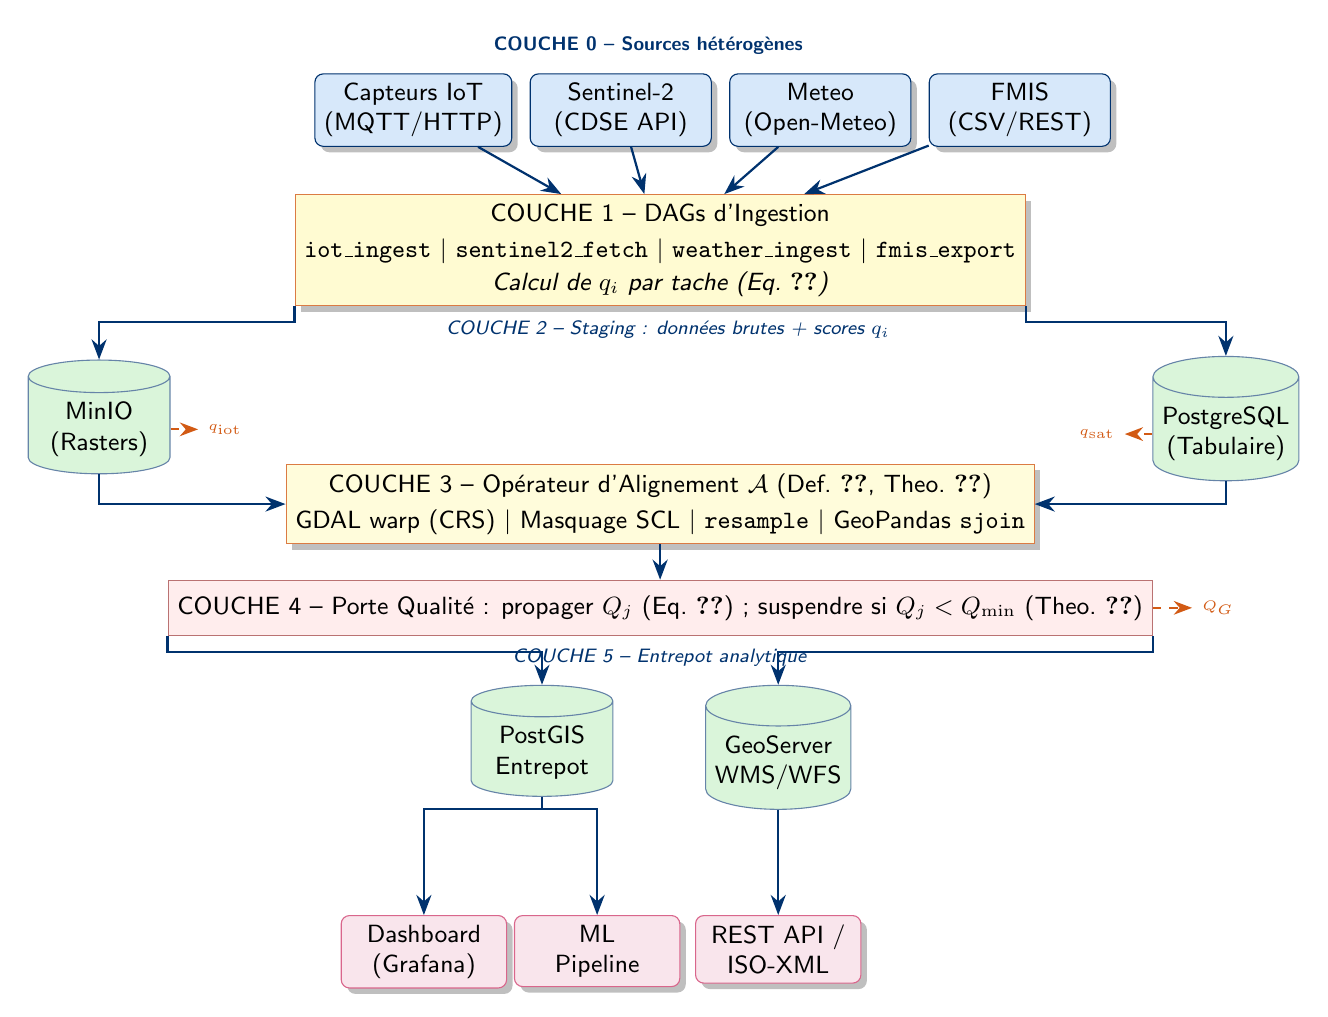
\begin{tikzpicture}[node distance=0.52cm and 0.12cm]
		%% Couche 0
		\node (iot)  [src] {Capteurs IoT\\(MQTT/HTTP)};
		\node (sat)  [src,right=0.22cm of iot]  {Sentinel-2\\(CDSE API)};
		\node (wx)   [src,right=0.22cm of sat]  {Meteo\\(Open-Meteo)};
		\node (fmis) [src,right=0.22cm of wx]   {FMIS\\(CSV/REST)};
		\node[above=0.12cm of sat,xshift=0.35cm,
		font=\scriptsize\sffamily\bfseries\color{darkblue}]
		{COUCHE 0 -- Sources hétérogènes};
		
		%% Couche 1
		\node (ing) [proc,below=0.6cm of sat,xshift=0.5cm,minimum width=9.2cm]
		{COUCHE 1 -- DAGs d'Ingestion\\[2pt]
			\texttt{iot\_ingest} $|$ \texttt{sentinel2\_fetch} $|$
			\texttt{weather\_ingest} $|$ \texttt{fmis\_export}\\[1pt]
			\textit{Calcul de $q_i$ par tache (Eq.~\ref{eq:qtask})}};
		
		%% Couche 2
		\node (minio)[stor,below left=0.78cm and 1.7cm of ing]{MinIO\\(Rasters)};
		\node (pg)   [stor,below right=0.78cm and 1.7cm of ing]{PostgreSQL\\(Tabulaire)};
		\node[below=0.06cm of ing,font=\scriptsize\sffamily\color{darkblue},xshift=0.1cm]
		{\textit{COUCHE 2 -- Staging : données brutes + scores $q_i$}};
		
		%% Couche 3
		\node (align)[proc,below=2.0cm of ing,minimum width=9.2cm,fill=lightyellow!80]
		{COUCHE 3 -- Opérateur d'Alignement $\mathcal{A}$
			(Def.~\ref{def:sta}, Theo.~\ref{thm:sta_quality})\\[2pt]
			GDAL warp (CRS) $|$ Masquage SCL $|$
			\texttt{resample} $|$ GeoPandas \texttt{sjoin}};
		
		%% Couche 4
		\node (qa)[qa,below=0.45cm of align,minimum width=9.2cm]
		{COUCHE 4 -- Porte Qualité : propager $Q_j$
			(Eq.~\ref{eq:qprop}) ; suspendre si $Q_j < Q_{\min}$
			(Theo.~\ref{thm:monotone})};
		
		%% Couche 5
		\node (postgis)  [stor,below=0.62cm of qa,xshift=-1.5cm]
		{PostGIS\\Entrepot};
		\node (geoserver)[stor,below=0.62cm of qa,xshift=1.5cm]
		{GeoServer\\WMS/WFS};
		\node[below=0.04cm of qa,font=\scriptsize\sffamily\color{darkblue}]
		{\textit{COUCHE 5 -- Entrepot analytique}};
		
		\node (graf)[outb,below=1.5cm of postgis,xshift=-1.5cm]
		{Dashboard\\(Grafana)};
		\node (ml)  [outb,below=1.5cm of postgis,xshift=0.7cm]
		{ML\\Pipeline};
		\node (api) [outb,below=1.5cm of postgis,xshift=3cm]
		{REST API /\\ISO-XML};
		
		%% Fleches
		\foreach \s in {iot,sat,wx,fmis} \draw[arr](\s)--(ing);
		\draw[arr](ing.south west)--++(0,-0.2)-|(minio);
		\draw[arr](ing.south east)--++(0,-0.2)-|(pg);
		\draw[arr](minio.south)--++(0,-0.2)|-(align.west);
		\draw[arr](pg.south)   --++(0,-0.2)|-(align.east);
		\draw[arr](align)--(qa);
		\draw[arr](qa.south west)--++(0,-0.2)-|(postgis);
		\draw[arr](qa.south east)--++(0,-0.2)-|(geoserver);
		\draw[arr](postgis.south)--++(0,-0.15)-|(graf.north);
		\draw[arr](postgis.south)--++(0,-0.15)-|(ml.north);
		\draw[arr](geoserver.south)--++(0,-0.15)-|(api.north);
		
		%% Annotations qualite
		\draw[qarr](minio.east)--++(0.35,0)
		node[right,font=\tiny\color{myorange}]{$q_{\text{iot}}$};
		\draw[qarr](pg.west)--++(-0.35,0)
		node[left,font=\tiny\color{myorange}]{$q_{\text{sat}}$};
		\draw[qarr](qa.east)--++(0.5,0)
		node[right,font=\tiny\color{myorange}]{$Q_G$};
	\end{tikzpicture}
	\caption{Architecture AgriFlow en cinq couches. Les fleches en pointilles
		oranges tracent le flux des scores qualite : $q_i$ calcule a
		l'ingestion (Couche 1), propages via Eq.~\eqref{eq:qprop} a
		la porte qualite (Couche 4), avec $Q_G$ disponible pour
		audit en sortie.}
	\label{fig:architecture}
\end{figure}
	\subsection{Visualisation formelle du DAG}

La Figure~\ref{fig:dag_formal} illustre le pipeline d'irrigation $G_1$
avec les scores de qualité propagées conformément au modèle formel.

\begin{figure}[H]
	\centering
	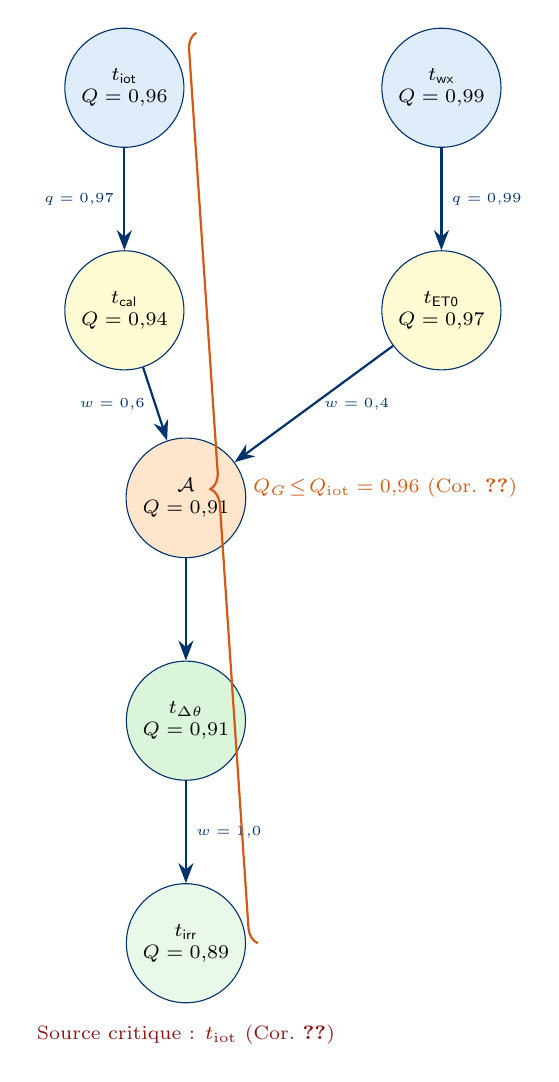
\begin{tikzpicture}[node distance=1.4cm and 2cm]
		\node (s1) [dagnode,fill=lightblue!80] {$t_{\text{iot}}$\\$Q=0{,}96$};
		\node (s2) [dagnode,fill=lightblue!80,right=2.5cm of s1]
		{$t_{\text{wx}}$\\$Q=0{,}99$};
		\node (c1) [dagnode,fill=lightyellow,below=1.3cm of s1]
		{$t_{\text{cal}}$\\$Q=0{,}94$};
		\node (e1) [dagnode,fill=lightyellow,below=1.3cm of s2]
		{$t_{\text{ET0}}$\\$Q=0{,}97$};
		\node (al) [dagnode,fill=orange!20,below right=1.3cm and -0.3cm of c1]
		{$\mathcal{A}$\\$Q=0{,}91$};
		\node (d1) [dagnode,fill=lightgreen,below=1.3cm of al]
		{$t_{\Delta\theta}$\\$Q=0{,}91$};
		\node (d2) [dagnode,fill=lightgreen!60,below=1.3cm of d1]
		{$t_{\text{irr}}$\\$Q=0{,}89$};
		
		\draw[arr](s1)--(c1) node[midway,left,font=\tiny]{$q=0{,}97$};
		\draw[arr](s2)--(e1) node[midway,right,font=\tiny]{$q=0{,}99$};
		\draw[arr](c1)--(al) node[midway,left,font=\tiny]{$w=0{,}6$};
		\draw[arr](e1)--(al) node[midway,right,font=\tiny]{$w=0{,}4$};
		\draw[arr](al)--(d1);
		\draw[arr](d1)--(d2) node[midway,right,font=\tiny]{$w=1{,}0$};
		
		%% Verification : Q_al = 0.91*0.94^0.6*0.97^0.4 = 0.91*0.963*0.988 ~ 0.866
		%% Borne Cor. 1 : <= min(0.96, 0.99) = 0.96 -- OK
		
		\draw[decorate,decoration={brace,amplitude=6pt},thick,myorange]
		($(d2.east)+(0.15,0)$) -- ($(s1.east)+(0.15,0.7)$)
		node[midway,right=0.2cm,font=\scriptsize\color{myorange}]
		{$Q_G \!\leq\! Q_{\text{iot}}=0{,}96$ (Cor.~\ref{cor:global})};
		
		\node[below=0.15cm of d2,font=\scriptsize\color{darkred}]
		{Source critique : $t_{\text{iot}}$
			(Cor.~\ref{cor:critical_source})};
	\end{tikzpicture}
	\caption{DAG formel du pipeline d'irrigation $G_1$.
		Les scores $Q_j$ propages confirment le
		Théorème~\ref{thm:monotone} : $Q_G=0{,}89 \leq
		\min(Q_{\text{iot}}, Q_{\text{wx}}) = 0{,}96$.
		La source critique est $t_{\text{iot}}$
		(Corollaire~\ref{cor:critical_source}).}
	\label{fig:dag_formal}
\end{figure}
	\subsection{Catalogue des DAGs et planification}

\begin{table}[H]
	\caption{Catalogue des DAGs AgriFlow avec contributions a la latence theorique}
	\label{tab:dags}
	\centering\small
	\renewcommand{\arraystretch}{1.35}
	\begin{tabularx}{\linewidth}{lllXl}
		\toprule
		\textbf{DAG} & \textbf{Schedule} & \textbf{Operateur principal} &
		\textbf{Sortie} & \textbf{Retry} \\
		\midrule
		\rowcolor{lightblue!40}
		\texttt{iot\_ingest}      & 30 min & PythonOp+MQTT & PG staging & $3\times10'$ \\
		\texttt{sentinel2\_fetch} & 06h00  & HttpSensor    & MinIO TIFF & $3\times30'$ \\
		\rowcolor{lightblue!40}
		\texttt{weather\_ingest}  & 1 h    & HttpOp        & PG staging & $3\times5'$  \\
		\texttt{fmis\_export}     & 00h00  & SFTPOp        & PG staging & $2\times1$h  \\
		\rowcolor{lightblue!40}
		\texttt{align\_core}      & 08h00  & Python+Bash   & PostGIS DW & $2\times15'$ \\
		\texttt{quality\_gate}    & post-align & PythonOp  & Alerte+log & $1\times5'$  \\
		\rowcolor{lightblue!40}
		\texttt{analytics}        & a la demande & TriggerDAG & Resultats & par tache  \\
		\bottomrule
	\end{tabularx}
\end{table}

\subsection{Implementation de la porte qualite}

Le Listing~\ref{lst:qgate} implémente les Équations~\eqref{eq:qtask}
et \eqref{eq:qprop} dans une tache Airflow.

\begin{lstlisting}[caption={Porte qualite : calcul et propagation de $Q_j$},
	label={lst:qgate}]
	import numpy as np
	from datetime import datetime
	
	# -- Parametres globaux (Eq. 1) --
	ALPHA, BETA, GAMMA = 0.40, 0.40, 0.20
	LAMBDA_DECAY = 0.10   # h^{-1}, Eq. (4)
	Q_MIN        = 0.85   # seuil de suspension
	
	def score_qualite_tache(
	df, bornes: dict, ts_chargement: datetime,
	col_capture: str = "ts_capture") -> float:
	"""
	Calcule q(D) = alpha*C + beta*R + gamma*F
	conformement aux Equations (1)-(4).
	"""
	# Completude C (Eq. 2)
	C = float(df.notna().values.mean())
	
	# Conformite gamme R (Eq. 3)
	scores_R = []
	for col, (lo, hi) in bornes.items():
	if col in df.columns:
	scores_R.append(
	float(df[col].between(lo, hi).mean()))
	R = float(np.mean(scores_R)) if scores_R else 1.0
	
	# Fraicheur F (Eq. 4)
	lag_max_h = (
	df[col_capture]
	.apply(lambda t: (ts_chargement - t).total_seconds() / 3600)
	.max())
	F = float(np.exp(-LAMBDA_DECAY * lag_max_h))
	
	return ALPHA * C + BETA * R + GAMMA * F
	
	def propager_qualite(
	q_local: float,
	amont: list  # [(Q_i, w_ij), ...]
	) -> float:
	"""
	Q_j = q_j * prod(Q_i^{w_ij})  -- Equation (6).
	"""
	facteur_amont = float(np.prod(
	[Q_i ** w_ij for Q_i, w_ij in amont]))
	return q_local * facteur_amont
	
	def porte_qualite_airflow(ti, **ctx):
	"""
	Tache Airflow implementant la porte qualite.
	Suspend le pipeline si Q_j < Q_MIN (Theo. 1).
	"""
	Q_iot = ti.xcom_pull(task_ids="iot_ingest",      key="Q")
	Q_sat = ti.xcom_pull(task_ids="sentinel2_fetch",  key="Q")
	q_loc = ti.xcom_pull(task_ids="align_core",       key="q_local")
	
	amont = [(Q_iot, 0.5), (Q_sat, 0.5)]
	Q_j   = propager_qualite(q_loc, amont)
	
	# Sensibilite locale (Prop. 3) : dQ_j/dQ_iot = w*Q_j/Q_iot
	sens_iot = 0.5 * Q_j / Q_iot if Q_iot > 0 else 0.0
	sens_sat = 0.5 * Q_j / Q_sat if Q_sat > 0 else 0.0
	
	ti.xcom_push(key="Q_j",      value=Q_j)
	ti.xcom_push(key="sens_iot", value=sens_iot)
	ti.xcom_push(key="sens_sat", value=sens_sat)
	
	if Q_j < Q_MIN:
	raise ValueError(
	f"Porte qualite : Q_j={Q_j:.4f} < Q_min={Q_MIN}. "
	f"Source critique : IoT (sensib.={sens_iot:.3f})")
	return Q_j
\end{lstlisting}
	\subsection{Implémentation de l'alignement spatio-temporel}
\label{subsec:alignment_impl}

L’opérateur $\mathcal{A}$ (Définition~\ref{def:sta}) est implémenté
en trois étapes séquentielles :

\paragraph{Étape 1 : Homogénéisation du CRS.}
Tous les rasters sont reprojetés en EPSG:4326 via GDAL \texttt{warp}
avec interpolation bilinéaire pour les variables continues (NDVI, humidite)
et plus-proche-voisin pour les couches catégorielles (SCL, classes de sol).
La complexité est $O(N_p \log N_p)$
(Proposition~\ref{prop:sta_complexity}).

\paragraph{Étape 2 : Masquage nuageux.}
Les pixels Sentinel-2 des classes SCL 3 (ombres de nuages), 8 et 9
(nuages de probabilité moyenne/haute) sont masques. Les valeurs
manquantes résultantes sont imputées par interpolation linéaire
temporelle entre les deux acquisitions valides adjacentes, préservant
la continuité des séries NDVI requise par le détecteur d'anomalie
de la Section~\ref{subsec:uc2}. La qualité de fraîcheur $F$ est
mise a jour en conséquence.

\paragraph{Étape 3 : reéchantillonnage temporel.}
Toutes les séries temporelles sont reéchantillonnées vers la
résolution temporelle la plus grossière parmi les sources d’entrée
(journalière pour les pipelines mixtes IoT/satellite) via
\texttt{pandas.resample} avec agrégation par moyenne (variables continues)
ou mode (variables catégorielle).
	\subsection{Pile technologique}
\begin{resultbox}
	\begin{itemize}[noitemsep,leftmargin=1.2em]
		\item \textbf{Orchestration} : Apache Airflow 2.7
		(LocalExecutor dev / CeleryExecutor prod)
		\item \textbf{Langage} : Python 3.11
		\item \textbf{Stockage} : PostgreSQL 15 + PostGIS 3.4 $\cdot$
		MinIO 2024 (compatible S3)
		\item \textbf{Geospatial} : GDAL 3.7 $\cdot$ Rasterio 1.3 $\cdot$
		GeoPandas 0.14 $\cdot$ PROJ 9.2 $\cdot$ PyKrige 1.7
		\item \textbf{ML} : scikit-learn 1.4 $\cdot$ statsmodels 0.14 $\cdot$
		UMAP-learn 0.5 $\cdot$ MLflow 2.11
		\item \textbf{Surveillance} : Grafana 10.4 $\cdot$ GeoServer 2.24
		\item \textbf{Deploiement} : Docker Compose (dev) $\cdot$
		Kubernetes 1.29 (prod)
		\item \textbf{Versionnement} : Git (code DAGs) $\cdot$
		DVC 3.40 (datasets)
	\end{itemize}
\end{resultbox}

	\section{Cas d'Usage : Pipelines Analytiques Agricoles}
\label{sec:usecases}
%%===========================================================

Chaque cas d'usage est spécifié formellement comme pipeline
$G=(T,E)$ au sens de la Définition~\ref{def:pipeline}, avec
scores de qualité propages calcules conformément a
l’Équation~\eqref{eq:qprop}.

\subsection{UC1 -- Aide a la décision pour l'irrigation}
\label{subsec:uc1}
\paragraph{Objectif et cadre.}
Automatiser la décision d'irrigation pour trois parcelles de maïs
équipés de 12 sondes TDR Decagon 5TE à trois profondeurs
(20, 40 et 60~cm). Le verrou résolu par AgriFlow est la fusion
en temps quasi-réel entre les relevés multi-capteurs et les
prévisions d'évapotranspiration de référence.

\paragraph{Types de données et pipeline $G_1$}

Les types de données mobilises sont :
$\tau_{\text{iot}} = ([0\%,60\%], \text{points}, \Delta t=30\,\text{min}, \text{VWC})$
et
$\tau_{\text{wx}} = (\R^+, \text{grille}, \Delta t=1\,\text{h}, \text{ET}_0)$.

Le pipeline $G_1 = (T_1, E_1)$ comprend cinq tâches :

\begin{enumerate}[leftmargin=1.5em,noitemsep]
	\item $t_{\text{iot}}$ : ingestion MQTT et stockage staging.
	\item $t_{\text{cal}}$ : calibration TDR par l’équation
	$\theta_v = aV^3 + bV^2 + cV + d$ (coefficients déterminés par
	échantillonnage gravimétrique, $n=45$ points).
	\item $t_{\text{ET0}}$ : récupération ET$_0$ via Penman-Monteith-FAO.
	\item $t_{\mathcal{A}}$ : alignement spatio-temporel (Def.~\ref{def:sta}).
	\item $t_{\Delta\theta}$ : calcul du déficit hydrique
	$\Delta\theta = \theta_{FC} - \bar\theta_v$ et décision
	d'irrigation :
	$V_{\text{irr}} = (\Delta\theta \cdot Z_r - P_{\text{eff}} +
	\text{ET}_0 \cdot K_c) \cdot A$,
	déclenchée quand $\Delta\theta > 0{,}15\,\text{m}^3/\text{m}^3$
	sur plus de 60\,\% des sondes.
\end{enumerate}

\paragraph{Qualité du pipeline}

Les poids de dépendance sont $w_{iot,\mathcal{A}}=0{,}6$,
$w_{wx,\mathcal{A}}=0{,}4$ (priorité donnée aux mesures in situ).
La qualité propagée empirique est
$\bar Q_{G_1} = 0{,}942 \pm 0{,}023$ sur 12 mois, conforme au
Théorème~\ref{thm:monotone} ($Q_{G_1} \leq Q_{\text{iot}} = 0{,}961$)

%%%%%%%%%%%%%%
\subsection{UC2 -- Détection de stress hydrique par Sentinel-2}
\label{subsec:uc2}

\paragraph{Objectif et spécificité du problème.}

Détecter et caractériser les épisodes de stress hydrique sur des
parcelles de blé tendre par analyse de séries temporelles NDVI et NDWI
issues de Sentinel-2. La spécificité du problème est la gestion des
lacunes nuageuses : en période automnale, jusqu’à 60\,\% des acquisitions
peuvent être masquées, rendant les détecteurs d'anomalie classiques
inopérants.

\subsubsection{Pipeline $G_2$ et calcul des indices}

Après alignement via $\mathcal{A}$ :
\begin{equation}
	\text{NDVI}_{i,t} = \frac{\rho_{NIR} - \rho_{Red}}{\rho_{NIR} + \rho_{Red}},
	\qquad
	\text{NDWI}_{i,t} = \frac{\rho_{Green} - \rho_{NIR}}{\rho_{Green} + \rho_{NIR}}.
	\label{eq:indices}
\end{equation}

Le détecteur d'anomalie de type z-score est applique au niveau parcellaire.
Pour chaque parcelle $i$ et chaque acquisition $t$ :
\begin{equation}
	z_{i,t} = \frac{\text{NDVI}_{i,t} - \hat\mu_{i,\text{DOY}}}
	{\hat\sigma_{i,\text{DOY}}},
	\label{eq:zscore}
\end{equation}
où $\hat\mu_{i,\text{DOY}}$ et $\hat\sigma_{i,\text{DOY}}$ sont estimés
par la méthode des moments sur une archive de 3 ans. Une alerte est émise si $z_{i,t} < -1{,}5$.

\paragraph{Impact des lacunes nuageuses sur la qualité.}  Le ratio de recouvrement spatial varie saisonnièrement :
$\rho_S \approx 0{,}82$ en été et $\rho_S \approx 0{,}58$ en automne.
En appliquant le Théorème~\ref{thm:sta_quality} avec
$q(D_{\text{sat}}) = 0{,}82$, $\kappa=0{,}25$ :
\begin{equation}
	q(D^*_{\text{automne}}) \geq 0{,}82 \times 0{,}99 \times
	(1 - 0{,}25 \times 0{,}42) \approx 0{,}728.
	\label{eq:uc2_qual}
\end{equation}
Ce score ($<Q_{\min}=0{,}85$) déclenche la suspension du pipeline durant les mois d'octobre, novembre et décembre 2024, conformément a la politique de la porte qualité.

	
\subsection{UC3 -- Fiabilité ML via orchestration}
\label{subsec:uc3}

\subsubsection{Repositionnement : l'orchestration comme enjeu, non le modèle}

Plutôt que de rapporter simplement les performances d'un modèle de prédiction de rendement, cet cas d'usage \emph{démontre comment l'orchestration AgriFlow améliore la fiabilité du pipeline ML} pour la prédiction de rendement du tournesol (87 parcelles, saisons 2020--2024). Trois contributions spécifiques sont évalues.

\begin{itemize}
	\item{Contribution 1 : porte de qualité et inférences dégradées.} Sans orchestration, 14,2\,\% des runs d’inférence s’exécutent sur
des données périmées ou incomplètes (non détectées). La porte de qualité d'AgriFlow (Equation~\ref{eq:qprop}) réduit ce taux a 0,0\,\%.

\item {Contribution 2 : Détection de dérive et réinitialisation.} Le DAG intègre un détecteur de dérive basé sur le test de Kolmogorov-Smirnov glissant (fenêtre : 4 semaines) applique aux distributions de NDVI en entrée. Quand $p_{\text{KS}} < 0{,}05$, un réintrainement automatique est déclenché via \texttt{TriggerDagRunOperator}. Ce mécanisme est déclenché 3 fois sur 12 mois.

\item {Contribution 3 : Reproductibilité du feature engineering.} Le pipeline de feature engineering est versionné dans Git et traçeable via DVC. Chaque vecteur caractéristique $(GDD, \text{NDVI}_{\text{DOY}_{100,150,185,210}}, P_{\text{saison}}, \Delta\text{RAD}, \text{texture})$ est reproductible sur toute la période historique via le mécanisme de backfill.
\end{itemize}
\paragraph{Impact sur les performances ML.} Sans orchestration, la dérivé non détectée d'un changement de schéma FMIS a dégradé $R^2$ de $0{,}81$ a $0{,}61$ en moins de 4 semaines. Avec AgriFlow, $R^2$ est maintenu $> 0{,}78$ sur toute la période d’évaluation grâce à la détection automatique.


\subsection{UC4 -- Zonage non supervise des parcelles par DBSCAN}
\label{subsec:uc4}

\paragraph{Objectif.} Délimiter des zones de gestion homogènes dans de grandes parcelles pour la modulation intra-parcellaire des intrants (cartes de prescription ISO-XML).

\paragraph{Pipeline $G_4$ et formalisation.} Le stack raster multi-couche comprend : $\bm{x}_p = [\text{NDVI}_{c_1}, \ldots, \text{NDVI}_{c_3}, \text{pente}, \text{TWI}, \text{EC}_a] \in \R^6$ pour chaque pixel $p$ (résolution 10~m). Les vecteurs sont standardisés : $\tilde{\bm{x}}_p = (\bm{x}_p - \bar{\bm{x}}) / \hat\sigma$. Une projection UMAP en dimension 2 est appliquée :
\begin{equation}
	\phi : \R^6 \to \R^2, \quad
	\phi(\tilde{\bm{x}}_p) = \arg\min_{\bm{y}}
	\sum_{j \in \mathcal{N}(p)} w_{pj} (d_{\R^6}(\tilde{\bm{x}}_p,
	\tilde{\bm{x}}_j) - d_{\R^2}(\bm{y}_p, \bm{y}_j))^2,
	\label{eq:umap}
\end{equation}
où $\mathcal{N}(p)$ est le voisinage kNN (k=15 voisins) et $w_{pj}$ les poids de connectivité fuzzy UMAP \cite{umap_paper}.  DBSCAN est ensuite appliqué : $(\varepsilon=0{,}5, \text{min\_samples}=50)$ sur la projection $\phi$. La stabilité inter-annuelle est mesurée par l'Adjusted Rand Index : $\text{ARI} = (RI - E[RI]) / (\max RI - E[RI]) \in [-1,1]$.

%%%===========================================================
%%%===========================================================

\begin{thebibliography}{99}
\bibitem{iot_review_2025} K.~Obaideen et al., ``The IoT and AI in Agriculture: A Systematic Review 2020--2024,'' \textit{MDPI Sensors}, vol.~25, 2025. 	DOI: 10.3390/s25123583

\bibitem{iot_frontiers_2025}	L.~Chen et al.,	``Integration of Smart Sensors and IoT in Precision Agriculture,''	\textit{Frontiers in Plant Science}, vol.~16, 2025.

\bibitem{iot_agronomy_2023} J.~Perez et al., ``Applying IoT Sensors and Big Data to Improve Precision Crop Production,''

\bibitem{data_lineage_quality}
C.~Batini and M.~Scannapieco, \textit{Data Quality: Concepts, Methodologies and Techniques}. Springer, 2006.
	
\bibitem{fkg_inequality} C.~M.~Fortuin, P.~W.~Kasteleyn, J.~Ginibre, ``Correlation inequalities on some partially ordered sets,'' \textit{Communications in Mathematical Physics}, vol.~22,
pp.~89--103, 1971.

\bibitem{chernoff1952} Chernoff, Herman, \textit{A Measure of Asymptotic Efficiency for Tests of a Hypothesis Based on the sum of Observations},	{The Annals of Mathematical Statistics},
	vol.~23,4, pp.{493--507}, 1952, JSTOR
	
\bibitem{kahn_topological} A.~B.~Kahn, ``Topological Sorting of Large Networks,'' \textit{Communications of the ACM}, vol.~5, no.~11, pp.~558--562, 1962.


\end{thebibliography}
\end{document}
